\documentclass{report}
\usepackage{graphicx, tikz-cd, float, titlepic, booktabs} % Required for inserting images
\usepackage{pgfplots}
\pgfplotsset{compat=1.15}
\usepackage{mathrsfs}
\usetikzlibrary{arrows}
\usepackage{amsmath, amssymb, amsthm, amsfonts, siunitx, physics, gensymb}
\AtBeginDocument{\RenewCommandCopy\qty\SI}
\usepackage[version=4]{mhchem}
\usepackage[most,many,breakable]{tcolorbox}
\usepackage{xcolor, fancyhdr, varwidth}
\usepackage[Glenn]{fncychap}
%Options: Sonny, Lenny, Glenn, Conny, Rejne, Bjarne, Bjornstrup
\usepackage{hyperref, cleveref}
\usepackage{icomma, enumitem} %comma as decimal and continue enumerate with [resume]
\usepackage{plimsoll} %use standard state symbol with \stst
\usepackage[danish]{babel}
%%%%%%%%%%%%%%%%%%%%%%%%%%%%%%
% SELF MADE COLORS
%%%%%%%%%%%%%%%%%%%%%%%%%%%%%%
\definecolor{myg}{RGB}{56, 140, 70}
\definecolor{myb}{RGB}{45, 111, 177}
\definecolor{myr}{RGB}{199, 68, 64}
\definecolor{mytheorembg}{HTML}{F2F2F9}
\definecolor{mytheoremfr}{HTML}{00007B}
\definecolor{mylenmabg}{HTML}{FFFAF8}
\definecolor{mylenmafr}{HTML}{983b0f}
\definecolor{mypropbg}{HTML}{f2fbfc}
\definecolor{mypropfr}{HTML}{191971}
\definecolor{myexamplebg}{HTML}{F2FBF8}
\definecolor{myexamplefr}{HTML}{88D6D1}
\definecolor{myexampleti}{HTML}{2A7F7F}
\definecolor{mydefinitbg}{HTML}{E5E5FF}
\definecolor{mydefinitfr}{HTML}{3F3FA3}
\definecolor{notesgreen}{RGB}{0,162,0}
\definecolor{myp}{RGB}{197, 92, 212}
\definecolor{mygr}{HTML}{2C3338}
\definecolor{myred}{RGB}{127,0,0}
\definecolor{myyellow}{RGB}{169,121,69}
\definecolor{myexercisebg}{HTML}{F2FBF8}
\definecolor{myexercisefg}{HTML}{88D6D1}
%%%%%%%%%%%%%%%%%%%%%%%%%%%%%%%%%%%%%%%%%%%%%%%%%%%%%%%%%%%%%%%%%%%%%%
% Box environments for theorems and problems
%%%%%%%%%%%%%%%%%%%%%%%%%%%%%%%%%%%%%%%%%%%%%%%%%%%%%%%%%%%%%%%%%%%%%
\setlength{\parindent}{1cm}
%================================
% Question BOX
%================================
\makeatletter
\newtcbtheorem{question}{Opgave}{enhanced,
	breakable,
	colback=white,
	colframe=myb!80!black,
	attach boxed title to top left={yshift*=-\tcboxedtitleheight},
	fonttitle=\bfseries,
	title={#2},
	boxed title size=title,
	boxed title style={%
			sharp corners,
			rounded corners=northwest,
			colback=tcbcolframe,
			boxrule=0pt,
		},
	underlay boxed title={%
			\path[fill=tcbcolframe] (title.south west)--(title.south east)
			to[out=0, in=180] ([xshift=5mm]title.east)--
			(title.center-|frame.east)
			[rounded corners=\kvtcb@arc] |-
			(frame.north) -| cycle;
		},
	#1
}{def}
\makeatother
%================================
% DEFINITION BOX
%================================

\newtcbtheorem[]{Definition}{Definition}{enhanced,
	before skip=2mm,after skip=2mm, colback=red!5,colframe=red!80!black,boxrule=0.5mm,
	attach boxed title to top left={xshift=1cm,yshift*=1mm-\tcboxedtitleheight}, varwidth boxed title*=-3cm,
	boxed title style={frame code={
					\path[fill=tcbcolback]
					([yshift=-1mm,xshift=-1mm]frame.north west)
					arc[start angle=0,end angle=180,radius=1mm]
					([yshift=-1mm,xshift=1mm]frame.north east)
					arc[start angle=180,end angle=0,radius=1mm];
					\path[left color=tcbcolback!60!black,right color=tcbcolback!60!black,
						middle color=tcbcolback!80!black]
					([xshift=-2mm]frame.north west) -- ([xshift=2mm]frame.north east)
					[rounded corners=1mm]-- ([xshift=1mm,yshift=-1mm]frame.north east)
					-- (frame.south east) -- (frame.south west)
					-- ([xshift=-1mm,yshift=-1mm]frame.north west)
					[sharp corners]-- cycle;
				},interior engine=empty,
		},
	fonttitle=\bfseries,
	title={#2},#1}{def}
\newtcbtheorem[]{definition}{Definition}{enhanced,
	before skip=2mm,after skip=2mm, colback=red!5,colframe=red!80!black,boxrule=0.5mm,
	attach boxed title to top left={xshift=1cm,yshift*=1mm-\tcboxedtitleheight}, varwidth boxed title*=-3cm,
	boxed title style={frame code={
					\path[fill=tcbcolback]
					([yshift=-1mm,xshift=-1mm]frame.north west)
					arc[start angle=0,end angle=180,radius=1mm]
					([yshift=-1mm,xshift=1mm]frame.north east)
					arc[start angle=180,end angle=0,radius=1mm];
					\path[left color=tcbcolback!60!black,right color=tcbcolback!60!black,
						middle color=tcbcolback!80!black]
					([xshift=-2mm]frame.north west) -- ([xshift=2mm]frame.north east)
					[rounded corners=1mm]-- ([xshift=1mm,yshift=-1mm]frame.north east)
					-- (frame.south east) -- (frame.south west)
					-- ([xshift=-1mm,yshift=-1mm]frame.north west)
					[sharp corners]-- cycle;
				},interior engine=empty,
		},
	fonttitle=\bfseries,
	title={#2},#1}{def}

\newtcbtheorem{theo}%
    {Theorem}{}{theorem}
\newtcolorbox{prob}[1]{colback=red!5!white,colframe=red!50!black,fonttitle=\bfseries,title={#1}}
%================================
% NOTE BOX
%================================

\usetikzlibrary{arrows,calc,shadows.blur}
\tcbuselibrary{skins}
\newtcolorbox{note}[1][]{%
	enhanced jigsaw,
	colback=gray!20!white,%
	colframe=gray!80!black,
	size=small,
	boxrule=1pt,
	title=\textbf{Note:},
	halign title=flush center,
	coltitle=black,
	breakable,
	drop shadow=black!50!white,
	attach boxed title to top left={xshift=1cm,yshift=-\tcboxedtitleheight/2,yshifttext=-\tcboxedtitleheight/2},
	minipage boxed title=1.5cm,
	boxed title style={%
			colback=white,
			size=fbox,
			boxrule=1pt,
			boxsep=2pt,
			underlay={%
					\coordinate (dotA) at ($(interior.west) + (-0.5pt,0)$);
					\coordinate (dotB) at ($(interior.east) + (0.5pt,0)$);
					\begin{scope}
						\clip (interior.north west) rectangle ([xshift=3ex]interior.east);
						\filldraw [white, blur shadow={shadow opacity=60, shadow yshift=-.75ex}, rounded corners=2pt] (interior.north west) rectangle (interior.south east);
					\end{scope}
					\begin{scope}[gray!80!black]
						\fill (dotA) circle (2pt);
						\fill (dotB) circle (2pt);
					\end{scope}
				},
		},
	#1,
}
%================================
% EXAMPLE BOX
%================================
\newtcbtheorem[number within=section]{Example}{Example}
{%
	colback = myexamplebg
	,breakable
	,colframe = myexamplefr
	,coltitle = myexampleti
	,boxrule = 1pt
	,sharp corners
	,detach title
	,before upper=\tcbtitle\par\smallskip
	,fonttitle = \bfseries
	,description font = \mdseries
	,separator sign none
	,description delimiters parenthesis
}
{ex}
%================================
% THEOREM BOX
%================================

\tcbuselibrary{theorems,skins,hooks}
\newtcbtheorem[number within=section]{Theorem}{Theorem}
{%
	enhanced,
	breakable,
	colback = mytheorembg,
	frame hidden,
	boxrule = 0sp,
	borderline west = {2pt}{0pt}{mytheoremfr},
	sharp corners,
	detach title,
	before upper = \tcbtitle\par\smallskip,
	coltitle = mytheoremfr,
	fonttitle = \bfseries\sffamily,
	description font = \mdseries,
	separator sign none,
	segmentation style={solid, mytheoremfr},
}
{th}

%%%%%%%%%%%%%%%%%%%%%%%%%%%%%%%%%%%%%%%%%%%%%%%%%%%%%%%%%%%%%%%%%
% SELF MADE COMMANDS
%%%%%%%%%%%%%%%%%%%%%%%%%%%%%%
\newcommand{\sol}{\setlength{\parindent}{0cm}\textbf{\textit{Løsning:}}\setlength{\parindent}{1cm}}
%%%%%%%%%%%%%%%%%%%%%%%%%%%%%%%%%
\usepackage[tmargin=2cm,rmargin=1in,lmargin=1in,margin=0.85in,bmargin=2cm,footskip=.2in]{geometry}\pagestyle{fancy}
\lhead{Minrui Kevin Zhou 3.b}
\rhead{Opgavesæt 5}

\title{Opgavesæt 5\\
{\Large \textbf{3.b kemi A}}}
\author{Kevin Zhou}
\date{\today}

\begin{document}
\maketitle
\begin{note}
  Databog fysik kemi (2007) er benyttet ved beregningerne.
\end{note}
\section*{Opgave 4 - Blåsyre}
\sol \\
\textbf{a.}
Da \ce{HCN} er en svag syre, så må der gælde, at 
\begin{equation*}
\begin{split}
  pH&=\frac{1}{2} \cdot \left(pK_s - \log\left(c_s\right) \right) \\
  &=\frac{1}{2} \cdot \left(-\log\left(\frac{4,90 \cdot 10 ^{-10}\;\unit{\textsc{m}}}{\unit{\textsc{m}} }  \right) - \log\left(\frac{0,125 \;\unit{\textsc{m}}}{\unit{\textsc{m}} } \right)\right) \\
  &\approx 5,11
\end{split}
\end{equation*}
I en $0,125 \;\unit{\textsc{m}} $ vandig opløsning af hydrogencyanid ved 25 °C har vi altså $pH=5,11$.\\[1ex]
\textbf{b.}
Vi beregner standard molar entropitilvækst $\Delta S \stst $ for reaktionen. 
\begin{equation*}
\begin{split}
  \Delta S \stst &= \left(S \stst \left(\ce{HCN(g)} \right) + 3 \cdot S \stst \left(\ce{H2(g)} \right) \right)  -\left(S \stst \left(\ce{CH4(g)}\right)  + S \stst \left(\ce{NH3(g)} \right) \right)\\
  &=\left(201,8 \;\unit{\frac{J}{mol \cdot K}} +3 \cdot 130,68 \;\unit{\frac{J}{mol \cdot K}}  \right) - \left(186,3 \;\unit{\frac{J}{mol \cdot K}} + 192,8 \;\unit{\frac{J}{mol \cdot K}} \right) \\
  &\approx 214,7 \;\unit{\frac{J}{mol \cdot K}} >0
\end{split}
\end{equation*}
Altså øges uordenen i reaktionen fra venstre mod højre.
Det er i overensstemmelse med, at antallet af gasmolekyler øges i den retning (der er 2 på venstre side af reaktionspilen og 4 på højre). \\[1ex]
\textbf{c.}
Siden der gælder, at 
\[
\Delta G \stst =-\Delta S \stst \cdot T+ \Delta H \stst 
\] 
så må der være en lineær sammenhæng mellem $\Delta G \stst $ og $T$ (for $\Delta H \stst $ og $\Delta S \stst $ kan regnes som konstante og temperaturuafhængige). 
Det giver da mening at lave en lineær regression, hvilket ses i \cref{fig:reg}.
Det ses, at punkterne ligger tilnærmelsesvist på den rette linje.
\begin{figure}[H]
\begin{center}
  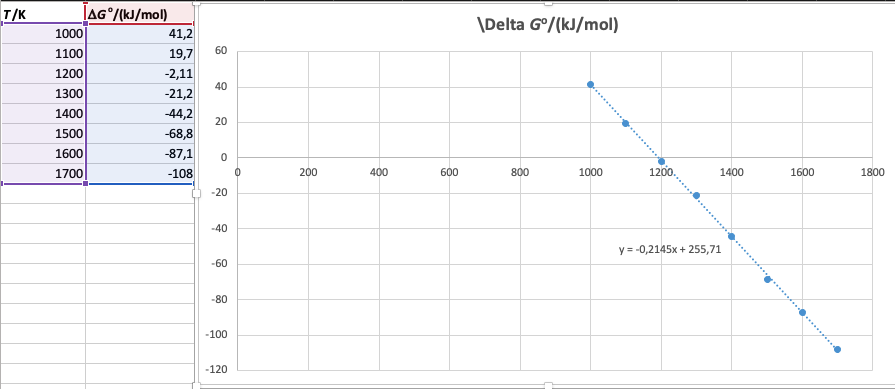
\includegraphics[width=\textwidth]{reg.png}
\end{center}
\caption{Lineær regression lavet i Excel}
\label{fig:reg}
\end{figure}
Fra regressionen har vi
\[
\Delta G \stst =-0,2145 \;\unit{\frac{kJ}{mol \cdot K}} \cdot T + 255,71 \;\unit{kJ/mol} 
\] 
Altså må den molare tilvækst i standard entalpi være 
\[
\Delta H \stst = 255,71 \;\unit{kJ/mol} >0
\] 
Reaktionen fra venstre mod højre er altså endoterm.
Det følger så fra Le Chateliers princip, at en forskydning mod højre sker, hvis temperaturen hæves.
Siden hydrogencyanid er på højre side af reaktionspilen, så skal temperaturen altså hæves for at øge udbyttet af hydrogencyanid.

For at finde ligevægtskonstantens enhed kigger vi på reaktionsbrøken for reaktionen fra venstre mod højre.
Denne er
\begin{equation*}
\begin{split}
  \frac{p(\ce{HCN} ) \cdot p(\ce{H2} )^3}{p(\ce{CH4} ) \cdot p(\ce{NH3})}
\end{split}
\end{equation*}
Siden enheden for partialtrykkene er bar, så må reaktionsbrøkens og ligevægtskonstantens enhed være 
\[
\frac{\unit{bar^4}}{\unit{bar^2}}=\unit{bar^2}
\] 
Vi kan nu udregne ligevægtskonstanten med van't Hoffs ligning ved $1000 \;\unit{\celsius} $.
\begin{equation*}
\begin{split}
  K&=e^{-\frac{\Delta H \stst }{R \cdot T} + \frac{\Delta S \stst }{R}} \;\unit{bar^2} \\
  &=e^{-\frac{255,71 \cdot 10^3\;\unit{J/mol} }{8,314 \;\unit{J/(mol \cdot K)} \cdot 1273,15 \;\unit{K}} + \frac{214,5 \;\unit{J/(mol \cdot K)} }{8,314 \;\unit{J/(mol \cdot K)}}} \;\unit{bar^2} \\
  &\approx 5,17 \;\unit{bar^2} 
\end{split}
\end{equation*}
Vi har altså ved $1000 \;\unit{\celsius} $ fået ligevægtskonstanten $K=5,17 \;\unit{bar^2} $ og temperaturen skal hæves for at øge udbyttet af hydrogencyanid.\\[1ex]
\textbf{d.}
For at beregne partialtrykkene ved ligevægt, opskrives et SÆL-skema, hvilket ses i \cref{tab:SÆL}.
\begin{table}[H]
\centering
\begin{tabular}{@{}llllll@{}}
\toprule
         & \ce{CH4(g) + } & \ce{NH3(g)} & \ce{<=>} & \ce{HCN(g) + } & \ce{3H2(g)} \\ \midrule
Start    & 0,35 bar           & 0,65 bar        &         & 0 bar              & 0 bar           \\
Ændring  & -x             & -x          &         & x              & 3x          \\
Ligevægt & 0,35 bar - x       & 0,65 bar - x    &         & x              & 3x          \\ \bottomrule
\end{tabular}
\caption{SÆL-skema for ligevægten}
\label{tab:SÆL}
\end{table}
Når ligevægten har indstillet sig, så må reaktionsbrøken være lig med ligevægtskonstanten:
\begin{equation*}
\begin{split}
  \frac{p(\ce{HCN} ) \cdot p(\ce{H2} )^3}{p(\ce{CH4} ) \cdot p(\ce{NH3})}=K &\iff \frac{x \cdot \left(3x\right)^3}{\left(0,35 \;\unit{bar} -x\right) \cdot \left(0,65 \;\unit{bar} -x\right)  }=5,1656 \;\unit{bar^2} \\
  &\iff x=-0,73106 \;\unit{bar}  \lor x=0,273 \;\unit{bar} 
\end{split}
\end{equation*}
Ligningen er løst med CAS (se \cref{fig:CAS}).
Kun den sidste løsning kan bruges, da den anden giver negative koncentrationer.
Vi kan nu udregne partialtrykkene.
\begin{equation*}
\begin{split}
  &p(\ce{CH4})=0,35 \;\unit{bar} - x=0,35 \;\unit{bar} - 0,273 \;\unit{bar} = 0,077 \;\unit{bar} \\
  &p(\ce{NH3} )=0,65 \;\unit{bar} - x=0,65 \;\unit{bar} - 0,273 \;\unit{bar} =0,377 \;\unit{bar} \\
  &p(\ce{HCN} )=x=0,273 \;\unit{bar} \approx 0,27 \;\unit{bar}  \\
  &p(\ce{H2} )=3x=3 \cdot 0,273 \;\unit{bar} =0,819 \;\unit{bar} 
\end{split}
\end{equation*}
Det samlede tryk i beholderen er blot summen af partialtrykkene.
\begin{equation*}
\begin{split}
  p&=p(\ce{CH4}) + p(\ce{NH3}) + p(\ce{HCN}) + p(\ce{H2})\\
  &=0,077 \;\unit{bar}  + 0,377 \;\unit{bar}  + 0,273 \;\unit{bar} + 0,819 \;\unit{bar} \\
  &\approx 1,5 \;\unit{bar} 
\end{split}
\end{equation*}
Altså har vi fået partialtrykket af hydrogencyanid til $p(\ce{HCN} )=0,27 \;\unit{bar} $ og det samlede tryk beholderen til at være $p=1,5 \;\unit{bar} $. 
\begin{figure}[H]
\begin{center}
  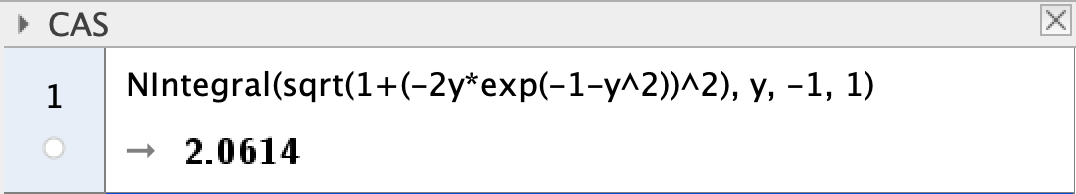
\includegraphics[width=\textwidth]{CAS.png}
\end{center}
\caption{Ligningen løses med CAS}
\label{fig:CAS}
\end{figure}
\section*{Opgave 1 - Parfume og allergi}
\sol \\
\textbf{a.}
Vi betragter først de funktionelle grupper (dobbeltbindinger tælles her som en funktionel gruppe), hvor stoffet A har to: en dobbeltbinding og en hydroxygruppe.
Hydroxygruppen har den højeste prioritet af de to, og navnet skal da ende på -ol. 
Vi nummererer af samme grund også \ce{C}-atomerne på den længste carbonkæde fra enden med hydroxygruppen (se \cref{fig:navn}).
\begin{figure}[H]
\begin{center}
  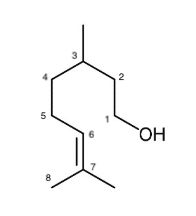
\includegraphics[width=0.5\textwidth]{navn.png}
\end{center}
\caption{\ce{C}-atomerne nummereret i strukturformlen for stoffet}
\label{fig:navn}
\end{figure}
Vi ser, at den længste kæde af \ce{C}-atomer er 8 lang, altså skal -oct- indgå i navnet.
De to methylgrupper på \ce{C}-atom nummer 3 og 7 angives med præfikset 3,7-dimethyl-, og dobbeltbindingen ved \ce{C}-atom nummer 6 (den mindste vælges altid) angives med suffikset -6-en.

Det systematiske navn for stof A må altså være 3,7-dimethyloct-6-en-1-ol.\\[1ex]
\textbf{b.}
Resultater for de tre kemiske tests (bromvand, Fehlings og drejning af planpolariseret lys) ses i hhv. \cref{fig:bromvand}, \cref{fig:fehling} og \cref{fig:lys}.
Bemærk, at det unumererede reagensglas længst til venstre er et kontrolforsøg.
\begin{figure}[H]
\begin{center}
  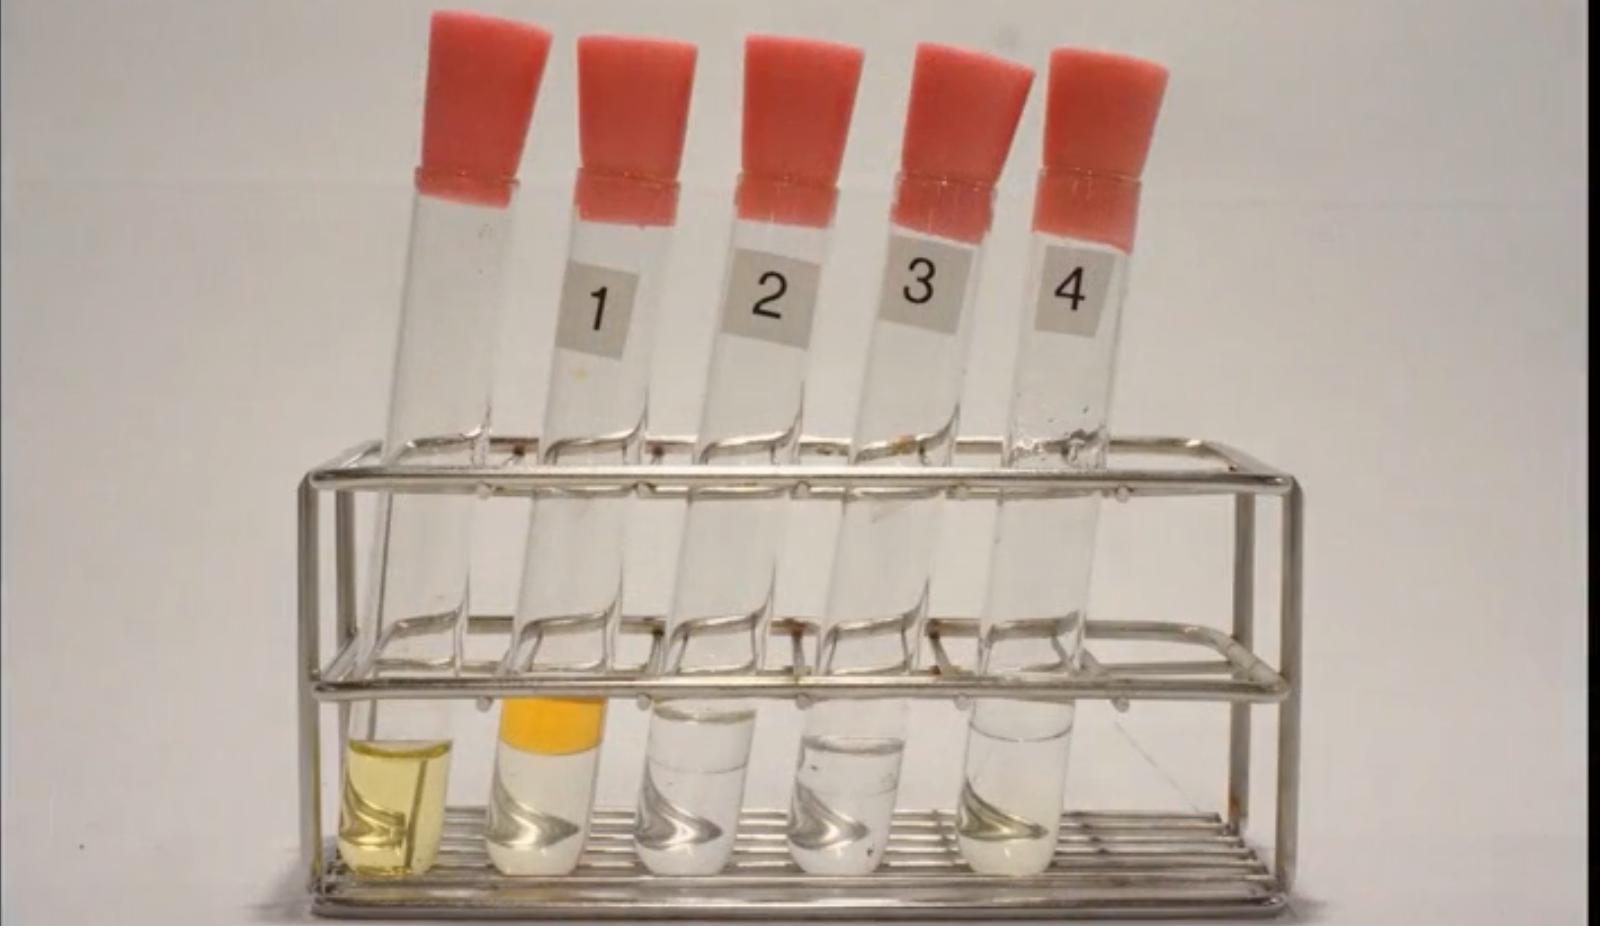
\includegraphics[width=\textwidth]{bromvand.png}
\end{center}
\caption{Kemisk test med bromvand}
\label{fig:bromvand}
\end{figure}
\begin{figure}[H]
\begin{center}
  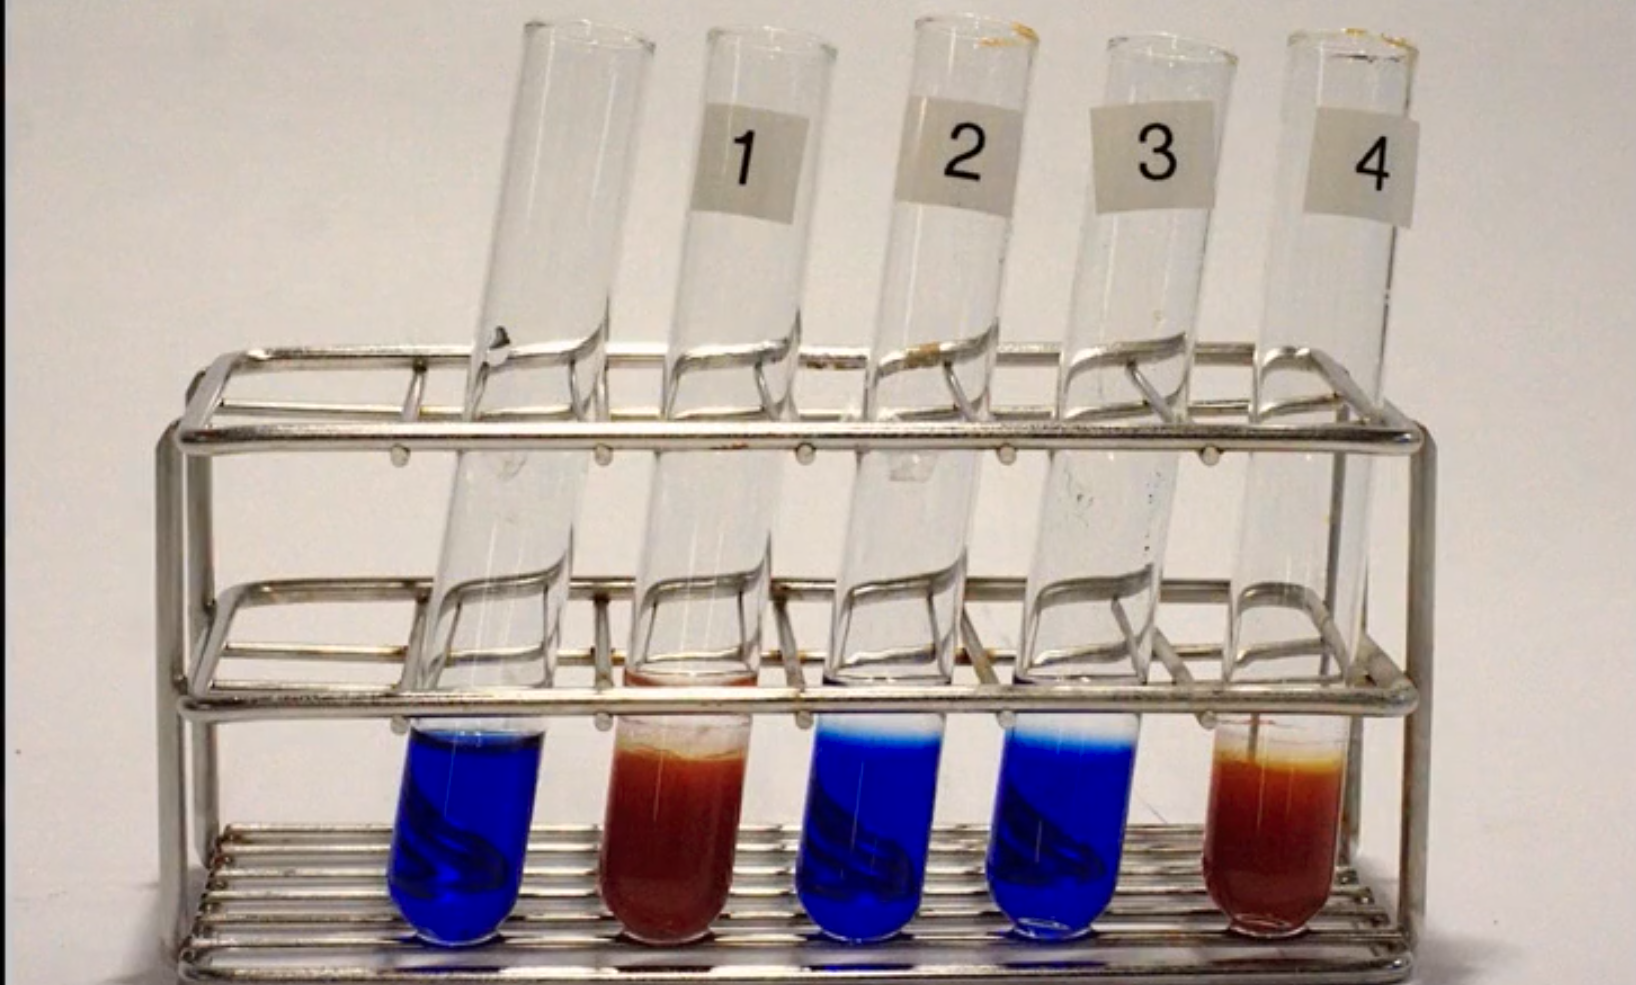
\includegraphics[width=\textwidth]{fehling.png}
\end{center}
\caption{Kemisk test med Fehlings væske}
\label{fig:fehling}
\end{figure}
\begin{figure}[H]
\begin{center}
  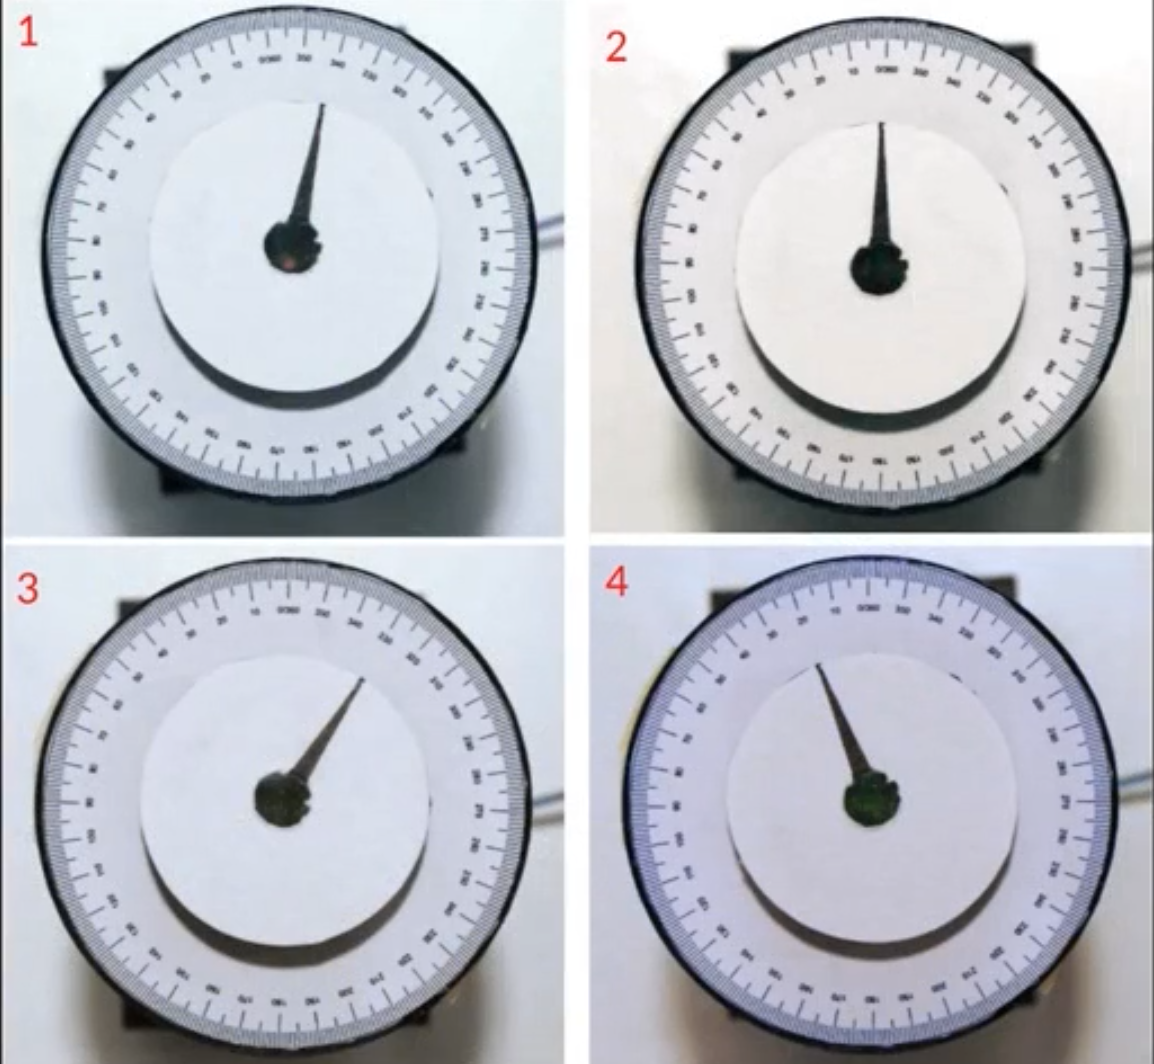
\includegraphics[width=0.5\textwidth]{planpolariseret.png}
\end{center}
\caption{Kemisk test med planpolariseret lys}
\label{fig:lys}
\end{figure}
Stoffer, der kan affarve bromvand, dvs. addere dibrom, er umættede.
I \cref{fig:bromvand} ser vi, at kun stoffet i reagensglas 1 ikke reagerer.
I \cref{fig:ABCD} er alle bindinger, der kan sprænges for at addere dibrom markeret med en gul cirkel, og det ses, at kun stof B ikke kan addere dibrom.
Altså må stof B være i reagensglas 1.

Som udgangspunkt danner kun aldehyder bundfald ved Fehlings prøve.
I \cref{fig:fehling} ses det, at der kun er udfældning i glas 1 og 4.
I \cref{fig:ABCD} er alle aldehydgrupper markeret med en blå cirkel, og det ses, at kun stof B og C er aldehyder.
Siden vi allerede ved, at B er i glas 1, så må stof C være i glas 4.

Et stof er optisk aktivt hvis og kun hvis det ikke er symmetrisk.
Fra \cref{fig:lys} har vi, at stofferne i glas 1,3 og 4 drejer planpolariseret lys, hvor stoffet i glas 2 ikke gør.
I \cref{fig:ABCD} er alle assymetriske \ce{C}-atomer markeret med en asterix, og det ses, at kun stof D ikke indholder et assymetrisk \ce{C}.
Altså må stof D være i glas 2. 
Med udelukkelsesprincippet må stof A så være i glas 3.

Vi har altså fået, at stof A er i glas 3, stof B i glas 1, stof C i glas 4 og stof D i glas 2.
\begin{figure}[H]
\begin{center}
  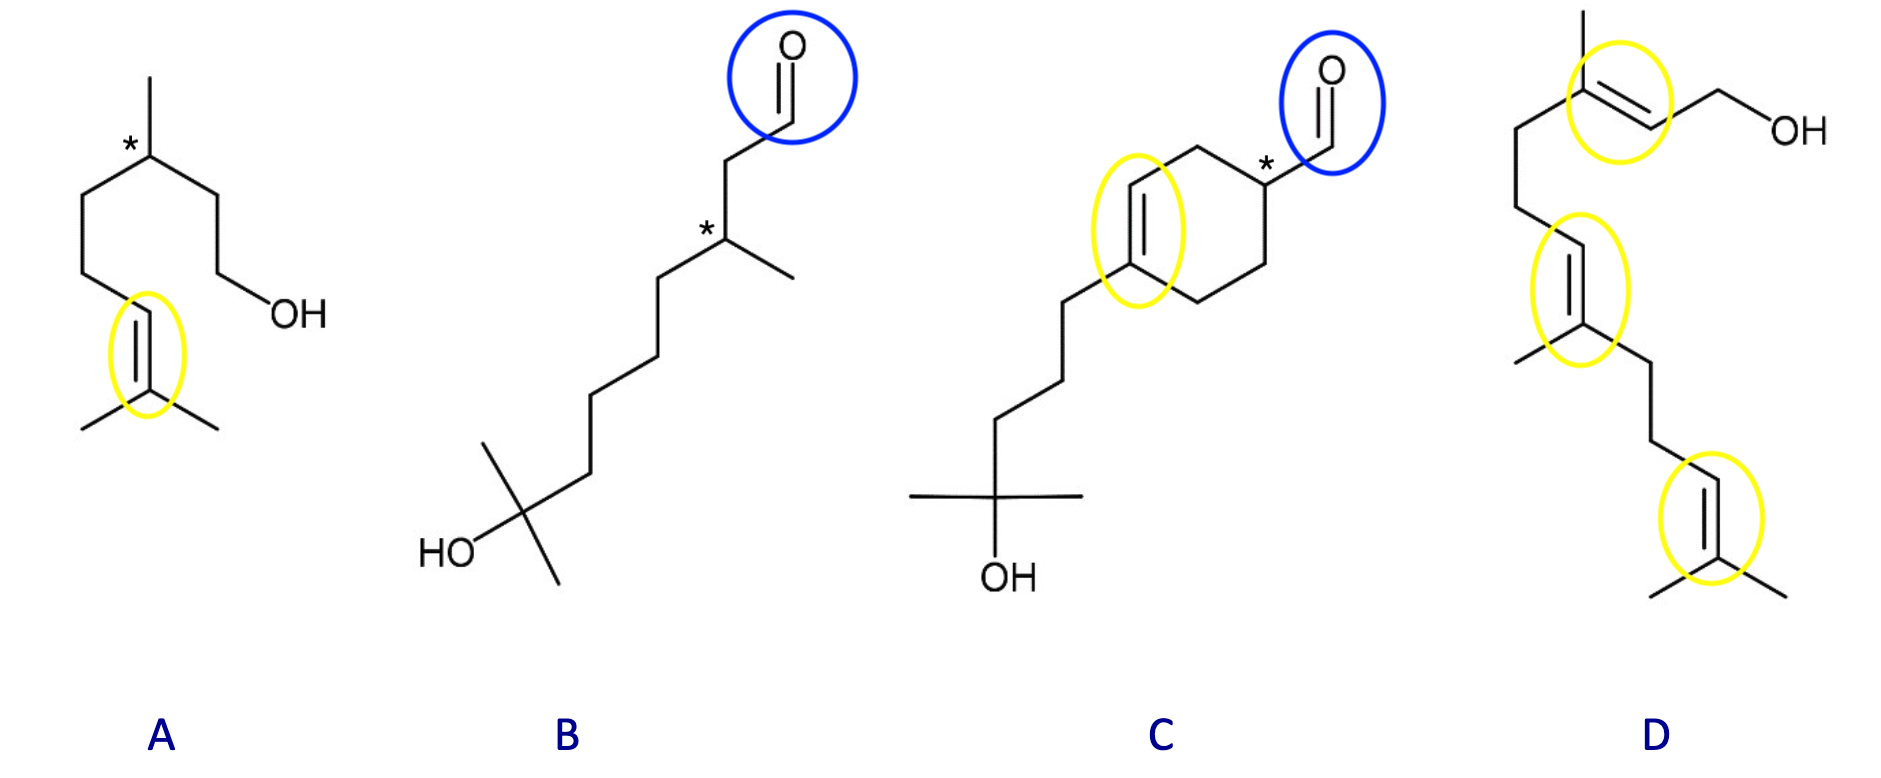
\includegraphics[width=\textwidth]{ABCD.png}
\end{center}
\caption{Markeringer på stoffere A, B, C og D}
\label{fig:ABCD}
\end{figure}
\noindent \textbf{c.}
Da molekylformlem \ce{C14H18O3} er kendt, kan man beregne DBE for stoffet:
\[
DBE=\frac{\left(2 \cdot 14 + 2\right) - \left(18-0\right) }{2}=6
\] 
Dette passer med, at stoffet indholder en aromatisk ring (4 DBE), endnu en ringslutning (1 DBE) samt et dobbeltbundet O i carbonylgruppen (1 DBE).
Altså er der ingen dobbeltbindingsækvivalenter i R.

Tilordningen af signalerne i spektret ses i \cref{tab:NMR}.
\begin{table}[H]
\centering
\begin{tabular}{@{}llllllll@{}}
\toprule
Signal & \begin{tabular}[c]{@{}l@{}}Aflæst kemisk skift\\ $\delta /\unit{ppm}$\end{tabular} & Integralforhold & \begin{tabular}[c]{@{}l@{}}Ækvivalente \\ $^1\ce{H}$-kerner\end{tabular} & Opsplitning & \begin{tabular}[c]{@{}l@{}}Antal \\ nabo-$^1\ce{H}$'er\end{tabular} & Tilordning & \begin{tabular}[c]{@{}l@{}}Kemisk skift\\ (tabelværdi)\\ $\delta/\unit{ppm}$\end{tabular} \\ \midrule
1      & 0,60                                                                               & 3               & 3                                                                   & triplet     & 2                                                              &        \ce{C\textbf{H}3-CH2}     &                                                                            0,9               \\
  2      & 1,22                                                                               & 6               & 6                                                                   & singlet     & 0                                                              &           \ce{(C\textbf{H}3)2-C}  &                                                                                       0,9    \\
3      & 1,59                                                                               & 2               & 2                                                                   & kvartet     & 3                                                              &           \ce{C\textbf{H}2-CH3-C}  &                                                                                        1,3   \\
4      & 4,62                                                                               & 2               & 2                                                                   & singlet     & 0                                                              &           \ce{C-C\textbf{H}2-O-Ar}  &                                                                          4,3                 \\
5      & 4,67                                                                               & 2               & 2                                                                   & singlet     & 0                                                              &            \ce{C-C\textbf{H}2-O-Ar}&                                                                                         4,3  \\
6      & 6,85                                                                               & 1               & 1                                                                   & dublet      & 1                                                              &           \ce{Ar-H}  &                                                                          6,5-8                 \\
7      & 6,95                                                                               & 1               & 1                                                                   & singlet     & 0                                                              &            \ce{Ar-H}&                                                                                          6,5-8 \\
8      & 7,19                                                                               & 1               & 1                                                                   & dublet      & 1                                                              &           \ce{Ar-H} &                                                                                  6,5-8         \\ \bottomrule
\end{tabular}
\caption{Tilordning af signaler i spektret}
\label{tab:NMR}
\end{table}
Med oplysningerne fra tabellen kan en strukturformel for stoffet og R tegnes, hvilket ses i \cref{fig:R}, hvor \ce{H}-atomerne er nummereret ift. de tilsvarende signaler i spektret, og R er markeret med en blå cirkel.
\begin{figure}[H]
\begin{center}
  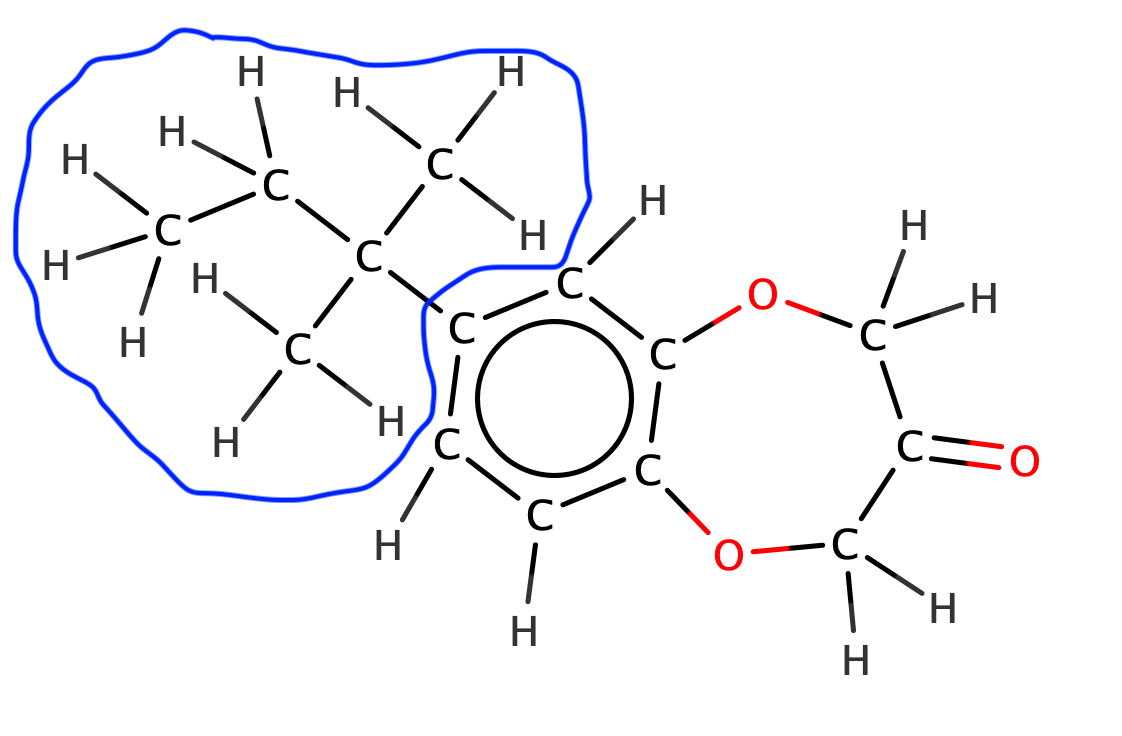
\includegraphics[width=\textwidth]{R.png}
\end{center}
\caption{Strukturformlen for stoffet, R er markeret med cirkel}
\label{fig:R}
\end{figure}
\section*{Opgave 2 - Vanadium}
\sol \\
\textbf{a.}
Da rent fast stof udelades i reaktionsbrøken, så må reaktionsbrøken for reaktionen fra venstre mod højre være
\[
\frac{p(\ce{Cl2} )}{p(\ce{VCl4} )^2}
\] 
\textbf{b.}
Da partialtrykkene har enheden bar, så må reaktionsbrøken og dermed ligevægtskonstanten have enheden
\[
\frac{\unit{bar}}{\unit{bar^2}}= \;\unit{bar^{-1}} 
\] 
Fra figuren får vi, at 
\begin{equation*}
\begin{split}
  \ln\left(K\right) =12773 \;\unit{K} \cdot \frac{1}{T}-29,8 \implies K= e^{\frac{12773 \;\unit{K}}{T}-29,8 } \;\unit{bar^{-1}} 
\end{split}
\end{equation*}
Vi kan nu regne $K$ ud ved $165 \;\unit{\celsius} $, hvilket svarer til $438,15 \;\unit{K} $. 
\begin{equation*}
\begin{split}
  K&= e^{\frac{12773 \;\unit{K}}{438,15 \;\unit{K} }-29,8 } \;\unit{bar^{-1}} \\
  &\approx 0,523 \;\unit{bar^{-1}} 
\end{split}
\end{equation*}
hvilket var, hvad vi ville vise. \\[1ex]
\textbf{c.}
Siden der fra van't Hoffs ligning gælder
\begin{equation*}
\begin{split}
  \ln\left(K\right) = - \frac{\Delta H \stst }{R}\cdot \frac{1}{T} + \frac{\Delta S \stst }{R}
\end{split}
\end{equation*}
og vi fra figuren har at
\begin{equation*}
\begin{split}
\ln\left(K\right) =12773 \;\unit{K} \cdot \frac{1}{T}-29,8 
\end{split}
\end{equation*}
så må det gælde, at
\begin{equation*}
\begin{split}
  &\Delta H \stst = -R \cdot 12773 \;\unit{K} =-8,314 \;\unit{\frac{J}{mol \cdot K}} \cdot 12773 \;\unit{K} \approx -106 \;\unit{kJ/mol} <0 \\
  &\Delta S \stst = R \cdot \left(-29,8\right) =8,314 \;\unit{\frac{J}{mol \cdot K}} \cdot \left(-29,8\right) \approx -248 \;\unit{\frac{J}{mol \cdot K}} <0
\end{split}
\end{equation*}
Da $\Delta H \stst <0$, så er reaktionen fra venstre mod højre endoterm.
Da $\Delta S \stst <0$, så øges ordenen fra venstre mod højre.
Det er i overensstemmelse med, at to gasmolekyler bliver til to faste partikler og ét gasmolekyle.\\[1ex]
\textbf{d.}
Vi beregner først den molare masse for vanadiumtetrachlorid.
\begin{equation*}
\begin{split}
  M(\ce{VCl4} )&=M(\ce{V} ) + 4 \cdot M(\ce{Cl})\\
  &=50,94 \;\unit{g/mol} + 4 \cdot 35,45 \;\unit{g/mol} \\
  &=192,74 \;\unit{g/mol} 
\end{split}
\end{equation*}
Vi beregner nu partialtrykket af vanadiumtetrachlorid til start med idealgasloven.
\begin{equation*}
\begin{split}
  p(\ce{VCl4} )&=\frac{n(\ce{VCl4} ) \cdot R \cdot T}{V}\\
  &=\frac{m(\ce{VCl4}) \cdot R \cdot T}{V \cdot M(\ce{VCl4} )}\\
  &=\frac{10,0 \;\unit{g} \cdot 0,0831 \;\unit{\frac{L \cdot bar}{mol \cdot K}} \cdot 438,15 \;\unit{K} }{2,00 \;\unit{L} \cdot 192,74 \;\unit{g/mol} }\\
  &=0,944544 \;\unit{bar} 
\end{split}
\end{equation*}
For at beregne gassernes sammensætning når ligevægten er indstillet, opstilles et SÆL-skema, hvilket ses i \cref{tab:SÆL2}.
\begin{table}[H]
  \centering
  \begin{tabular}{@{}lllll@{}}
    \toprule
    & \ce{2VCl4(g)}  & \ce{<=>} & \ce{2VCl3(s) +} & \ce{Cl2(g)} \\
    \midrule
    Start & 0,944544 bar & &  & 0 bar \\
    Ændring & $-2x$ & &  & $x$\\
    Ligevægt & $0,944544 \;\unit{bar} - 2x$ & &  & $x$ \\
    \bottomrule
  \end{tabular}
  \caption{SÆL-skema}
  \label{tab:SÆL2}
\end{table}
Ved ligevægt er reaktionsbrøken lig med ligevægtskonstanten:
\begin{equation*}
\begin{split}
  \frac{p(\ce{Cl2} )}{p(\ce{VCl4} )^2}=K &\iff \frac{x}{(0,944544 \;\unit{bar} -2x)^2}=0,523 \;\unit{bar^{-1}} \\
  &\iff x=0,17942 \;\unit{bar}  \lor x=1,24314 \;\unit{bar} 
\end{split}
\end{equation*}
som er løst med CAS (se \cref{fig:CAS2}).
Kun den første løsning kan bruges, da den anden giver negatiive koncentrationer.
Vi kan nu beregne partialtrykkene for dichlor og vanadiumtetrachlorid.
\begin{equation*}
\begin{split}
  &p(\ce{Cl2} )=x=0,17942 \;\unit{bar} \approx 0,179 \;\unit{bar} \\
  &p(\ce{VCl4} )=0,944544 \;\unit{bar} -2x = 0,9944544 \;\unit{bar} - 2 \cdot 0,17942 \;\unit{bar} \approx 0,586 \;\unit{bar} 
\end{split}
\end{equation*}
Når ligevægten er indstillet ved $165 \;\unit{\celsius} $, så er altså $p(\ce{Cl2} )=0,179 \;\unit{bar} $ og $p(\ce{VCl4} )=0,586 \;\unit{bar} $. 
\begin{figure}[H]
\begin{center}
  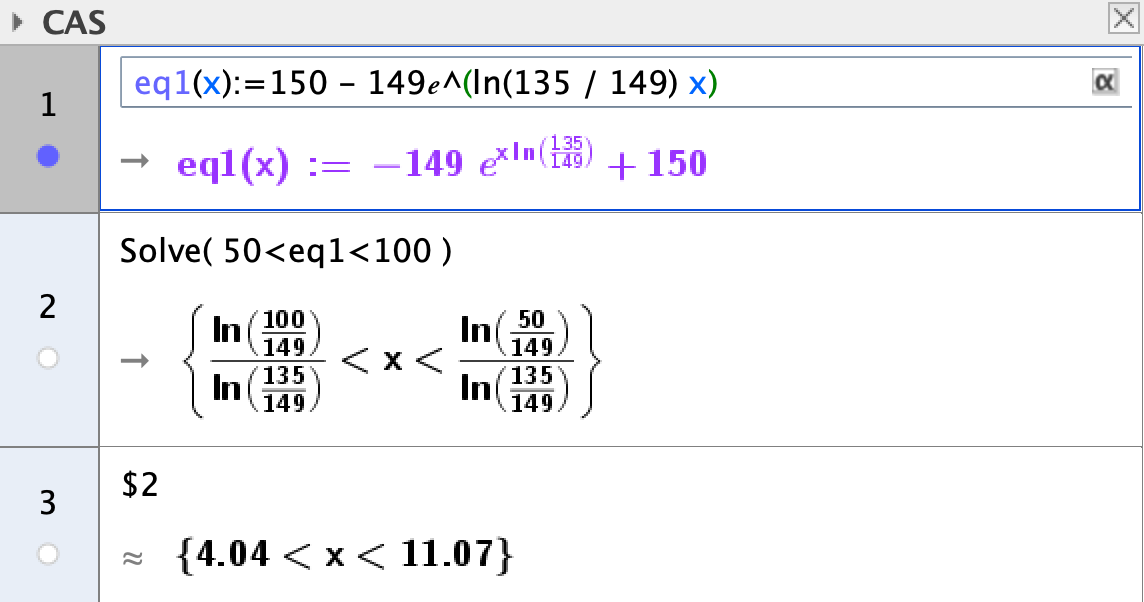
\includegraphics[width=\textwidth]{CAS2.png}
\end{center}
\caption{Ligningen løst mht. $x$ med CAS }
\label{fig:CAS2}
\end{figure}

\end{document}
